\documentclass[conference]{IEEEtran}
\IEEEoverridecommandlockouts

\usepackage{cite}
\usepackage{amsmath,amssymb,amsfonts}
\usepackage{graphicx}
\usepackage{textcomp}
\usepackage{xcolor}
\usepackage{booktabs}
\usepackage{array}
\usepackage{url}
% Character protrusion and font expansion. Materially improves justification in
% IEEEtran's narrow two-column measure, which is where nearly all the
% underfull-box warnings came from.
\usepackage{microtype}
\usepackage[hidelinks]{hyperref}

\graphicspath{{../figures/}}
% Measured figures come from the generated macro file, not retyped, so the
% two manuscripts cannot drift apart from each other or from the harness.
% Generated by run_all.py from named measurement records.
\newcommand{\RepeatThreeSpeed}{196.4}
\newcommand{\RepeatThreePower}{204.6}
\newcommand{\RepeatThreeTime}{1.61}
\newcommand{\RepeatThreeEnergy}{0.091}
\newcommand{\RepeatThreeMin}{0.078}
\newcommand{\RepeatThreeMax}{0.094}
\newcommand{\RepeatThreeMilliWh}{0.30}
\newcommand{\RepeatThreeHostZero}{0.091}
\newcommand{\RepeatThreeHostThirty}{0.12}
\newcommand{\RepeatThreeHostSixty}{0.13}
\newcommand{\RepeatThreeHostHundred}{0.15}
\newcommand{\RepeatEightSpeed}{102.5}
\newcommand{\RepeatEightPower}{222.2}
\newcommand{\RepeatEightTime}{3.09}
\newcommand{\RepeatEightEnergy}{0.19}
\newcommand{\RepeatEightMin}{0.17}
\newcommand{\RepeatEightMax}{0.20}
\newcommand{\RepeatEightMilliWh}{0.63}
\newcommand{\RepeatEightHostZero}{0.19}
\newcommand{\RepeatEightHostThirty}{0.24}
\newcommand{\RepeatEightHostSixty}{0.27}
\newcommand{\RepeatEightHostHundred}{0.31}
\newcommand{\RtxThreeSpeed}{195.6}
\newcommand{\RtxThreePower}{203.4}
\newcommand{\RtxThreeTime}{1.62}
\newcommand{\RtxThreeEnergy}{0.091}
\newcommand{\RtxThreeMin}{0.078}
\newcommand{\RtxThreeMax}{0.093}
\newcommand{\RtxThreeMilliWh}{0.30}
\newcommand{\RtxThreeHostZero}{0.091}
\newcommand{\RtxThreeHostThirty}{0.12}
\newcommand{\RtxThreeHostSixty}{0.13}
\newcommand{\RtxThreeHostHundred}{0.15}
\newcommand{\RtxEightSpeed}{101.8}
\newcommand{\RtxEightPower}{224.1}
\newcommand{\RtxEightTime}{3.11}
\newcommand{\RtxEightEnergy}{0.19}
\newcommand{\RtxEightMin}{0.18}
\newcommand{\RtxEightMax}{0.19}
\newcommand{\RtxEightMilliWh}{0.65}
\newcommand{\RtxEightHostZero}{0.19}
\newcommand{\RtxEightHostThirty}{0.24}
\newcommand{\RtxEightHostSixty}{0.27}
\newcommand{\RtxEightHostHundred}{0.31}
\newcommand{\AdaptationBaseAccuracy}{86.7}
\newcommand{\AdaptationAdaptedAccuracy}{97.8}
\newcommand{\AdaptationFrontierAccuracy}{95.0}
\newcommand{\AdaptationUplift}{11.1}
\newcommand{\AdaptationUpliftLow}{5.0}
\newcommand{\AdaptationUpliftHigh}{18.3}
\newcommand{\AdaptationClusterP}{0.250}
\newcommand{\AdaptationObservationCount}{300}
\newcommand{\AdaptationModelCount}{3}
\newcommand{\AdaptationExtractionBaseAccuracy}{100.0}
\newcommand{\AdaptationExtractionAdaptedAccuracy}{100.0}
\newcommand{\AdaptationExtractionUplift}{0.0}
\newcommand{\AdaptationExtractionP}{1.000}
\newcommand{\AdaptationExtractionAdjustedP}{1.000}
\newcommand{\AdaptationRagBaseAccuracy}{100.0}
\newcommand{\AdaptationRagAdaptedAccuracy}{100.0}
\newcommand{\AdaptationRagUplift}{0.0}
\newcommand{\AdaptationRagP}{1.000}
\newcommand{\AdaptationRagAdjustedP}{1.000}
\newcommand{\AdaptationSummaryBaseAccuracy}{91.7}
\newcommand{\AdaptationSummaryAdaptedAccuracy}{100.0}
\newcommand{\AdaptationSummaryUplift}{8.3}
\newcommand{\AdaptationSummaryP}{1.000}
\newcommand{\AdaptationSummaryAdjustedP}{1.000}
\newcommand{\AdaptationSimpleCodeBaseAccuracy}{91.7}
\newcommand{\AdaptationSimpleCodeAdaptedAccuracy}{100.0}
\newcommand{\AdaptationSimpleCodeUplift}{8.3}
\newcommand{\AdaptationSimpleCodeP}{1.000}
\newcommand{\AdaptationSimpleCodeAdjustedP}{1.000}
\newcommand{\AdaptationHardReasonBaseAccuracy}{50.0}
\newcommand{\AdaptationHardReasonAdaptedAccuracy}{88.9}
\newcommand{\AdaptationHardReasonUplift}{38.9}
\newcommand{\AdaptationHardReasonP}{0.250}
\newcommand{\AdaptationHardReasonAdjustedP}{1.000}
\newcommand{\AdaptationHoldoutBaseAccuracy}{80.0}
\newcommand{\AdaptationHoldoutAdaptedAccuracy}{90.0}
\newcommand{\AdaptationHoldoutFrontierAccuracy}{95.0}
\newcommand{\AdaptationHoldoutUplift}{10.0}
\newcommand{\AdaptationHoldoutUpliftLow}{5.0}
\newcommand{\AdaptationHoldoutUpliftHigh}{15.0}
\newcommand{\AdaptationHoldoutClusterP}{0.250}
\newcommand{\AdaptationSemanticBaseAccuracy}{90.3}
\newcommand{\AdaptationSemanticAdaptedAccuracy}{91.8}
\newcommand{\AdaptationSemanticFrontierAccuracy}{95.0}
\newcommand{\AdaptationSemanticUplift}{1.4}
\newcommand{\AdaptationSemanticUpliftLow}{-3.3}
\newcommand{\AdaptationSemanticUpliftHigh}{7.7}
\newcommand{\AdaptationSemanticClusterP}{1.000}


\definecolor{edgegreen}{HTML}{16A085}
\definecolor{edgedark}{HTML}{0E6E5C}
\definecolor{cloudorange}{HTML}{E8743B}
\definecolor{heavyred}{HTML}{C0392B}
\definecolor{accentblue}{HTML}{2F6FED}
\definecolor{ink}{HTML}{1F2933}

\newcommand{\Wh}{\,\text{Wh}}
\newcommand{\kWh}{\,\text{kWh}}
\newcommand{\fs}{f_{s}}
\newcommand{\pp}{\,\text{pp}}

\begin{document}

\title{Teaching at the Edge:\\
On-Device Parameter-Efficient Adaptation and\\
What It Actually Buys}

\author{\IEEEauthorblockN{AutoYou Research}
\IEEEauthorblockA{\textit{Decentralized Inference \& Sustainable Compute Group}\\
\texttt{research@autoyou.me}}
\thanks{Research release v0.3.0 (2026-09-14). Venue and DOI are not assigned in this version.}}

\maketitle

\begin{abstract}
A companion study evaluated local inference on consumer hardware, measuring
request-window GPU board energy of $\RtxThreeEnergy\Wh$ for 3B and $\RtxEightEnergy\Wh$ for 8B on an
RTX 5070, and replacing unconditional carbon, water and cost headlines with
explicit accounting boundaries and limits on cloud comparisons~\cite{autoyou2026edge}.
That study treated the small-model-sufficient workload fraction $\fs$ as fixed by
parameter count. This paper tests whether parameter-efficient fine-tuning (PEFT)
moves it, on hardware the household already owns. We model sixteen 2026-era
adaptation methods, three consumer device classes, and the memory, time, energy
and money cost of an adaptation run; we check the memory model against a
publicly documented 27B-parameter training run to within $-0.6\%$ and compare throughput
against the same run's wall clock. We state five hypotheses and three counter-claims.
Our central result is negative with respect to the obvious coverage hypothesis:
at the companion study's acceptance threshold $\alpha = 0.70$, the modelled
adaptation changes coverage by $\mathbf{+0.0\pp}$ - not at all, because every
adaptable task class already cleared the bar. This invariance is structural
conditional on the declared class ratios and workload weights. A public-safe
held-out evaluation across three models, five synthetic task classes, 20
evaluation tasks per class and three adapter-training seeds measures task
accuracy from $\AdaptationBaseAccuracy\%$ to $\AdaptationAdaptedAccuracy\%$,
a $+\AdaptationUplift\pp$ point estimate with a model-cluster bootstrap
interval of $\AdaptationUpliftLow$--$\AdaptationUpliftHigh\pp$. The exact
cluster sign-flip test is $p=\AdaptationClusterP$ with only three model
clusters, so this is evidence for the declared synthetic benchmark, not a
strong population-level significance claim. The earlier $+2/+6/+14$ points
and the derived $88.4\% \rightarrow 93.9\%$ figure remain exploratory
scenario inputs for routing sensitivity, not the measured quality result. The
measured benchmark is not a sampled user workload, a human quality study, or
an independent device replication. Coverage responds only above
$\alpha \approx 0.80$ in the exploratory scenario, and that threshold depends
on the uplift assumed. A single public recipe reports a 27B adaptation run;
applying its reported $130$\,W sustained package power to $82.1$ hours implies
$10.7\kWh$. Against an all-cloud counterfactual that is repaid in $143$ days of
ordinary use, but charging it only against the routing the adapter actually
changes - the correct attribution - it is never repaid at $\alpha = 0.70$,
because it moves no query, and takes $1.8$ to $3.3$ years where it does. We
report both bounds and record H8 as accounting-dependent rather than
validated. Repeating adaptation per user is scale-invariant under this model,
which answers the ``centralized training amortizes better'' objection on its own
terms. A private one-deployment report provides bounded, deployment-reported
observations: five rank-32 LoRA runs are reported as moving one task from
$30.8\%$ to $92.9\%$, while refusal of out-of-scope requests moved from $0\%$
to $100\%$ and source-code leakage from $25\%$ to $0\%$. The underlying
prompts, transcripts, checkpoints, and task-level labels are not redistributable
or independently auditable here, so these observations are not a population
estimate or a replacement for the planned experiment. They delimit, rather
than dispute, the literature concern that fine-tuning can degrade safety
alignment.
As a separate prompt-surface robustness probe, changing the surrounding
instructions while reusing the public evaluation records gives $80.0\%$ to
$90.0\%$ accuracy, or $+10.0\pp$ with a model-cluster interval of
$+5.0$--$+15.0\pp$ and exact $p=0.250$. This probe is not a new semantic
workload, an independent replication, or evidence that the primary effect
generalises beyond the released records.
A separate new-semantic holdout uses 100 fresh synthetic records, 20 per
class, with new record values and task formats. Across the same three model
clusters and three adapter seeds it gives $\AdaptationSemanticBaseAccuracy\%$
to $\AdaptationSemanticAdaptedAccuracy\%$, or only
$+\AdaptationSemanticUplift\pp$, with a model-cluster interval from
$\AdaptationSemanticUpliftLow\pp$ to
$+\AdaptationSemanticUpliftHigh\pp$ and exact $p=\AdaptationSemanticClusterP$.
The model-level directions are mixed, so this result weakens a broad
semantic-transfer reading of the primary uplift. It remains synthetic,
automatically graded, and measured on one physical host.
\end{abstract}

\begin{IEEEkeywords}
parameter-efficient fine-tuning, LoRA, QLoRA, edge computing, sustainable AI,
on-device training, privacy, small language models
\end{IEEEkeywords}

% ===================================================================== %
\section{Introduction}

The companion study~\cite{autoyou2026edge} asked whether it is feasible to
\emph{run} a small model at home. Measuring an NVIDIA RTX 5070 under Ollama at
499 input and 300 output tokens, it observed median request-window GPU board
energy of $\RtxThreeEnergy\Wh$ for 3B and $\RtxEightEnergy\Wh$ for 8B, while establishing that
environmental comparisons against cloud baselines remain conditional on workload
matching, task success, grid intensity and whole-system counterfactuals. Under an
assumed small-model-sufficient workload fraction $\fs \approx 82\%$, decentralised
execution trades off against cloud alternatives, but against a hyper-efficient
cloud model at $0.24\Wh$ per prompt~\cite{elsworth2025} a single consumer GPU
is worse once the comparison is made on like terms --- the board-rail figures
above exclude host draw and supply loss, whereas the cloud figure is a
comprehensive at-the-wall measurement --- and on genuinely hard reasoning a
small model is not a substitute at all.

Throughout, one quantity did the work. $\fs$ is computed from per-task-class
capability ratios - small-model quality divided by frontier quality - and
those ratios were treated as properties of parameter count. This paper asks
what happens when they are not.

Two things changed in 2026 that make the question answerable rather than
speculative. First, the open-weights tier a household can hold moved from 8B to
27B: Qwen3.8-27B~\cite{qwen38_2026} is dense, natively multimodal, Apache-2.0
licensed, and carries a 262K-token context. The official Ollama distribution
lists an $18$\,GB Q4\_K\_M build~\cite{qwen38_ollama2026}; that is distribution
metadata rather than a measurement of whole-system memory or runtime energy.
Second, consumer unified-memory APUs put $128$\,GB in front of the
accelerator, and a public recipe documents multi-day 27B LoRA training on one
of them~\cite{strixhalo2026}. Adapting a 27B model has therefore been
demonstrated outside data-centre hardware, although the recipe remains a
single community validation point.

Our contributions:

\begin{enumerate}
\item A \textbf{cost model for on-device adaptation} covering memory, wall
      clock, energy, carbon and money, checked against a publicly documented 27B run to
      $-0.6\%$ on peak memory (\S\ref{sec:model}).
\item A \textbf{conditional negative result on the obvious coverage hypothesis}:
      under the declared ratios, adaptation does not increase coverage at an
      ordinary acceptance threshold; a separate public synthetic benchmark
      measures task-accuracy change without claiming a real-workload effect
      (\S\ref{sec:uplift}).
\item An \textbf{amortisation analysis} charging the full training footprint
      against the inference it displaces, under two accountings that disagree
      by more than an order of magnitude, and a correction to our own earlier
      reading of it (\S\ref{sec:amortise}).
\item A \textbf{delimitation of the fine-tuning safety result}, supported by
      one deployment's reported runs (\S\ref{sec:safety}).
\item A \textbf{scale-invariance argument} against the
      centralized-amortisation objection (\S\ref{sec:scale}), and an explicit
      separation of which of our results are structural and which are inherited
      from an assumption (\S\ref{sec:whatisevidence}).
\end{enumerate}

All parametric models and figures are deterministically recomputed from
grounded equations and documented parameters; none is transcribed.

% ===================================================================== %
\section{The 2026 method roster}
\label{sec:roster}

Sixteen methods are modelled. They divide into families that behave very
differently on a memory-bound device, and the division matters more than any
individual method's reported gain.

Unless a sentence below is a definition of the method or a library
compatibility fact, the stated gain, speed, or forgetting property is an
author-reported result from the cited paper's own tasks and protocol. None of
these sixteen methods is re-run in this study. We use the reported ranges only
to bound a design sensitivity; they are not a matched ranking of methods on the
private deployment workload.

Every method below is a variant of low-rank adaptation~\cite{hu2021lora};
\cite{lorasurvey2024} surveys the family, and \cite{peft_library2026}
documents which of them sit one keyword argument away in the library a
household would actually use.

\textbf{Free.} \emph{rsLoRA}~\cite{kalajdzievski2023rslora} scales adapters by
$\alpha/\sqrt{r}$ instead of $\alpha/r$. This is one keyword argument with an
outsized effect: under the original scaling, raising the rank shrinks the
effective update, so higher ranks stop helping - which is why so much practice
settled on $r \in \{8,16\}$ and concluded that rank does not matter. It does;
the scaling was hiding it. \emph{LoRA+}~\cite{hayou2024loraplus} gives the two
factors different learning rates; its paper reports an infinite-width result
and faster convergence under its evaluated settings.
\emph{NEFTune}~\cite{jain2023neftune} adds embedding noise and reports its
largest gains on conversational quality specifically. None of the three costs
additional persistent adapter memory in our accounting; their training-time
overhead is not measured here.

\textbf{Initialisation.} \emph{PiSSA}~\cite{meng2024pissa} starts the adapter in
the principal singular subspace of $W$ rather than at noise-and-zero;
\emph{OLoRA}~\cite{buyukakyuz2024olora} uses QR-based orthonormal
initialisation; \emph{EVA}~\cite{paischer2024eva} runs a few batches of the
\emph{actual} dataset and allocates rank where that dataset needs it;
\emph{CorDA}~\cite{yang2024corda} can build the update in directions the base
model does not use for general knowledge. \emph{LoftQ}~\cite{li2023loftq}
initialises the adapter to absorb quantization error, so training does not begin
by repairing the damage quantization did. Their one-time initialization costs
are outside our measured adapter transport model; no recurring cost is claimed
here.

\textbf{Quantization.} \emph{QLoRA}~\cite{dettmers2023qlora} combines NF4,
double quantization of the block constants ($\approx 0.37$ bits per parameter),
and paged optimizer states. It is one route by which a 27B model can fit on
consumer hardware, but the fit and training-time tradeoff depend on context,
optimizer, checkpoint, and runtime. This study does not re-measure its wall
clock or memory profile.

\textbf{Reparameterisation.} \emph{DoRA}~\cite{liu2024dora} splits the update
into magnitude and direction; its paper reports larger gains at low rank in its
evaluated settings. That is a hypothesis for the edge, not an edge measurement.
\emph{AdaLoRA}~\cite{zhang2023adalora} reallocates a fixed rank budget across
layers during training. \emph{VeRA}~\cite{kopiczko2023vera} and
\emph{LoRA-XS}~\cite{balazy2024loraxs} go the other way, cutting trainable
parameters by over $100\times$ in a reported 7B comparison, with the quality
tradeoff depending on task and rank; \S\ref{sec:transport}
explains why that trade is interesting for a distributed product even when it is
uninteresting for a benchmark.

\textbf{Wrong shape.} \emph{GaLore}~\cite{zhao2024galore} reports a higher
continued-pretraining ceiling than LoRA in its evaluated settings, but it
updates all weights and therefore produces a new model rather than a mergeable
adapter. For a system whose distribution unit is a small personal delta, we
treat that shape as outside the adapter-only transport design regardless of
quality. We include it to make the criterion explicit: the artifact's
\emph{shape} is a first-order design constraint, not an implementation detail.

Fig.~\ref{fig:landscape} places all sixteen on cost against reported gain.

\begin{figure*}[t]
\centering
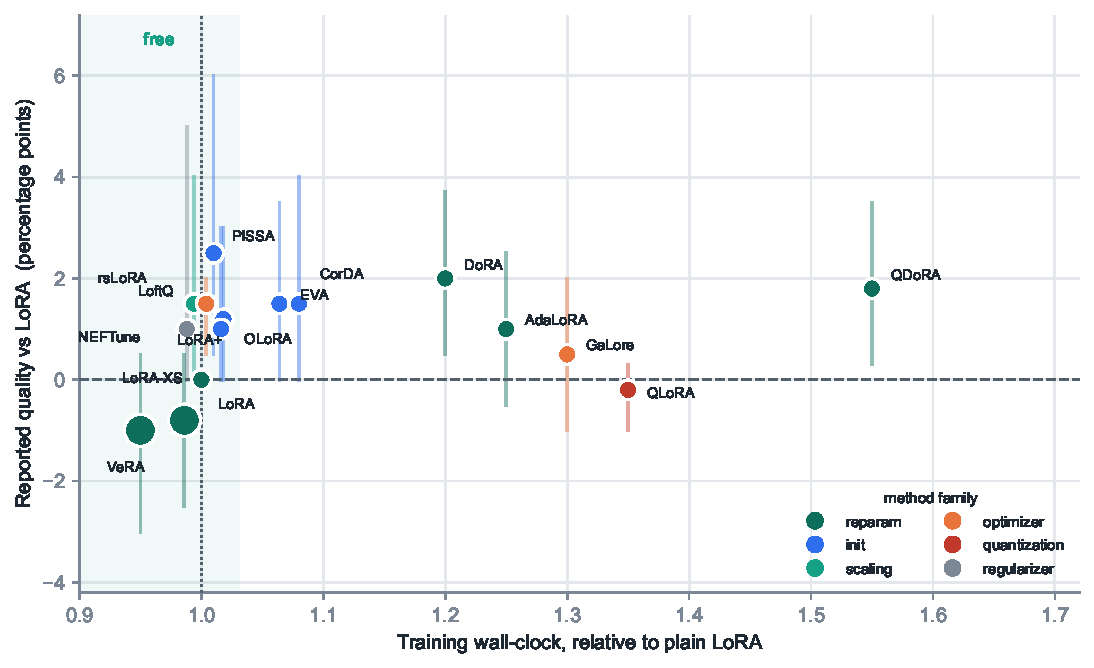
\includegraphics[width=\textwidth]{fig_method_landscape.pdf}
\caption{The 2026 roster. Vertical bars span each method's reported range
against a LoRA baseline; the dot is the modal reported gain; large dots shrink
the adapter by more than $20\times$. Three methods sit on the $1.0$ line:
reported gains at no wall-clock cost. Ranges are the methods' own authors'
benchmarks on their own tasks and are used here only to bound sensitivity.}
\label{fig:landscape}
\end{figure*}

% ===================================================================== %
\section{Cost model and validation}
\label{sec:model}

\subsection{Memory}

Peak accelerator memory for an adapter job is
\begin{equation}
M = \underbrace{P b_w}_{\text{weights}}
  + \underbrace{n_a(b_a + b_g + b_o)}_{\text{adapter, grads, optimizer}}
  + A + L + \varepsilon,
\end{equation}
where $P$ is the parameter count, $b_w$ the bytes per stored weight
($2$ for bf16, $4.127/8$ for NF4 with double quantization), $n_a$ the trainable
adapter parameters, $A$ the activation term, $L$ the logit term
$= B S V \cdot 4$ bytes, and $\varepsilon$ an $8\%$ allocator margin. With
gradient checkpointing,
$A = L_{\text{layers}} B S H \cdot 2 + B S H \cdot 34 \cdot 2$.

The logit term is easily overlooked and is not small: at $S = 8192$ over a
$152$K vocabulary it is $\approx 5$\,GB by itself, computed in fp32 for every
position.

\subsection{Validation}

One 27B run is publicly documented in enough detail to check against:
Qwen3.5-27B~\cite{qwen35_2026}, LoRA
$r = 128$, $\alpha = 256$, bf16 weights, paged 8-bit AdamW, sequence 8192, batch
1, gradient accumulation 4, on a 128\,GB unified-memory APU, reported at
$\approx 80$\,GB peak reserved~\cite{strixhalo2026}. Our model predicts
$\mathbf{79.5}$\,\textbf{GB}, a $-0.6\%$ residual, decomposing as $54.0$ weights,
$6.4$ adapter, gradients and optimizer combined, $8.2$ activations, $5.0$ logits, $5.9$
allocator.

\subsection{Time and energy}

Adapter training costs $\approx 6N$ FLOPs per token with checkpointing: $2N$
forward, $2N$ backward to activations (still required to reach earlier layers
even with frozen weights), $2N$ for the recomputed forward; the adapter's own
gradient is $O(n_a)$ and rounds away. The same publicly documented run gives
$448$ steps $\times$ $11$ minutes at $32{,}768$ tokens per step, from which the
achieved throughput is $\mathbf{8.04}$~TFLOP/s - a model-FLOPs utilisation of
$0.136$ against the part's $\approx 59$~TFLOP/s bf16 peak, and $49.6$ tokens per
second. At $130$\,W sustained package power the full run consumes
$\mathbf{10.7\kWh}$ over $82.1$ hours.

\subsection{Device class dominates}

\begin{table}[t]
\caption{Peak training memory, $r{=}128$, sequence 8192}
\label{tab:devices}
\centering
\small
\begin{tabular}{lrrr}
\toprule
& \textbf{dGPU 24\,GB} & \textbf{APU 128\,GB} & \textbf{NPU} \\
\midrule
Usable memory & 19\,GB & 102\,GB & 13\,GB \\
Bandwidth & 1008\,GB/s & 256\,GB/s & 120\,GB/s \\
Training power & 430\,W & 130\,W & -- \\
\midrule
27B bf16 & no & \textbf{yes} & no \\
27B 4-bit & $r{=}32$, $S{=}1024$ & \textbf{yes} & no \\
8B bf16 & yes & yes & no \\
\bottomrule
\end{tabular}
\end{table}

Table~\ref{tab:devices} states the paper's least intuitive result. The
\emph{faster} consumer device cannot adapt the larger model. A discrete GPU with
four times the memory bandwidth is driven down to rank 32 at sequence 1024
before a 27B job fits, while a unified-memory APU runs it at rank 128 and
sequence 8192 with $20$\,GB to spare. Bandwidth decides how quickly a run
finishes; addressable memory decides whether it can start.

This is why the companion study, which modelled only the discrete-GPU class,
had no way to reach the question this paper asks.

% ===================================================================== %
\section{Does adaptation move \texorpdfstring{$\fs$}{f\_s}?}
\label{sec:uplift}

\subsection{What can and cannot be adapted}

An adapter learns the shape of a distribution it was shown. It can learn how a
person phrases things, which of their files matter, what a product's screens are
called, and when to refuse. It cannot teach a small model competition
mathematics, because the training set contains no such capability to distil: the
ceiling on hard reasoning is the base model's depth, and PEFT does not raise it.
We therefore mark four of the five workload classes adaptable and hold
the hard-reasoning class fixed - which means the companion study's central negative
finding survives this paper unchanged.

The existing $+2$, $+6$ and $+14$ capability-ratio points (low, central, high)
are exploratory sensitivity inputs, not observed effects. They are retained
only to show how the routing arithmetic would respond to a bounded uplift, with
the pessimistic reading of Biderman \emph{et al.}~\cite{biderman2024lora} as
context rather than as a measured effect size. Ratios are capped at $0.99$: an
adapter may close the gap to a frontier model on a narrow task, but no claim is
made that a rank-32 update exceeds one. A new public multi-model, multi-task
evaluation replaces this scenario for the narrower estimand of held-out
synthetic task accuracy. It does not replace the real-workload sample, the
human grading plan, or the independent-device replication still needed for a
product-level claim.

\subsection{The result}

At $\alpha = 0.70$, $\fs$ is unchanged: $82\% \rightarrow 82\%$, a gain of
$+0.0\pp$. Every adaptable class already cleared the bar without adaptation, so
there is nothing for the uplift to recruit.

\textbf{H9 as stated remains only partially supported.} The public benchmark
measures held-out task accuracy, not the real-workload fraction $\fs$. Across
the declared $\AdaptationModelCount$ models and $\AdaptationObservationCount$
model-task observations, accuracy rises from $\AdaptationBaseAccuracy\%$ to
$\AdaptationAdaptedAccuracy\%$, a measured change of
$+\AdaptationUplift\pp$ (cluster bootstrap
$\AdaptationUpliftLow$--$\AdaptationUpliftHigh\pp$). The exact cluster
sign-flip test is $p=\AdaptationClusterP$: the direction is consistent across
the three model clusters, but three clusters do not support a strong
population-level significance claim. The gain is concentrated in hard-reasoning
tasks ($+\AdaptationHardReasonUplift\pp$); extraction and retrieval questions
are already at $\AdaptationExtractionAdaptedAccuracy\%$ and
$\AdaptationRagAdaptedAccuracy\%$ in this benchmark. This is a measured
synthetic-task result, not evidence
that a deployed assistant improves by the same amount.
The class-level effects are secondary: the hard-reasoning cluster test has
raw $p=\AdaptationHardReasonP$, and the five-test Bonferroni-adjusted value is
$p=\AdaptationHardReasonAdjustedP$; no task-class effect is confirmatory in
this three-cluster study.

\subsection{Prompt-surface robustness}

The primary benchmark's disjoint task identifiers do not by themselves show
that an adapter learned transferable semantics. We therefore ran a separate
probe on the same public evaluation records after changing the outer
instruction, class-specific wording, and labels surrounding the answer
choices. The probe assigns new task identifiers and uses the same three model
clusters, five classes, and three adapter-training seeds, but it deliberately
does not claim a new workload sample.

On this changed prompt surface, base accuracy is
$\AdaptationHoldoutBaseAccuracy\%$, adapted accuracy is
$\AdaptationHoldoutAdaptedAccuracy\%$, and the frontier reference is
$\AdaptationHoldoutFrontierAccuracy\%$. The adapted-minus-base change is
$+\AdaptationHoldoutUplift\pp$ with a model-cluster bootstrap interval of
$+\AdaptationHoldoutUpliftLow$--$+\AdaptationHoldoutUpliftHigh\pp$ and exact
two-sided cluster sign-flip $p=\AdaptationHoldoutClusterP$. The direction and
scale are similar to the primary result, which weakens the simplest objection
that the effect is caused only by the exact outer wording. It does not answer
the stronger objections: the underlying semantic records and answer labels
are reused, only one paraphrase is tested, contamination is not probed, and
the run remains on one physical host. The holdout is therefore a robustness
check, not an independent replication or a product-quality estimate.

\subsection{New-semantic holdout}

The prompt-surface probe above reuses semantic records, so we also generated
a separate holdout with new synthetic records, new domain values, and a
different reasoning format. It contains 20 tasks per class across extraction,
retrieval, summary, simple code, and hard reasoning. The released task
manifest has no primary evaluation task identifiers or source-task links, and
the runner records that primary prompts and answers are not copied. The same
three model clusters and three saved adapter-training seeds are scored with
the same blinded greedy four-choice grader.

On this new semantic holdout, base accuracy is
$\AdaptationSemanticBaseAccuracy\%$, adapted accuracy is
$\AdaptationSemanticAdaptedAccuracy\%$, and the frontier reference is
$\AdaptationSemanticFrontierAccuracy\%$. The adapted-minus-base change is
$+\AdaptationSemanticUplift\pp$, with a model-cluster bootstrap interval from
$\AdaptationSemanticUpliftLow\pp$ to
$+\AdaptationSemanticUpliftHigh\pp$ and exact two-sided cluster sign-flip
$p=\AdaptationSemanticClusterP$. The model-level changes are $+7.7$ pp,
$-3.3$ pp, and $0.0$ pp for the 0.5B, 3B, and VL 3B clusters respectively.
The mixed directions and interval spanning zero are counterevidence against
treating the primary $+11.1\pp$ as a broad semantic-transfer effect. This is
still a synthetic accuracy check on one host; it does not test contamination,
untouched general ability, human task success, sampled user work, or
independent-device reproducibility.

Under the central exploratory scenario, mean capability on the served workload
would rise from $88.4\%$ to $93.9\%$ of frontier, a derived gain of $+5.6\pp$
that closes $48\%$ of the remaining gap. Those values remain arithmetic
consequences of the scenario, not observations. In that same scenario,
coverage responds only above $\alpha \approx 0.80$,
where the unadapted model begins failing classes the adapted one still passes:
at $\alpha = 0.80$ coverage goes $70\% \rightarrow 82\%$, and at
$\alpha = 0.90$, $48\% \rightarrow 70\%$ (Fig.~\ref{fig:quality}).

\subsection{Which half of this result is evidence}
\label{sec:whatisevidence}
Those two numbers are not the same kind of claim, and conflating them is the
easiest way to misread this paper.

The \emph{coverage} result is algebraically invariant conditional on the
declared class partition, base ratios and workload weights. At $\alpha = 0.70$
every adaptable class already sits above the threshold, so no positive uplift
can recruit additional workload: we obtain $\fs = 82\%$ for every uplift tested
from $0$ to $+30$ points. It does not establish that a sampled user workload
has those ratios or weights; a task corpus with classes near the threshold
could change the result.

The \emph{measured synthetic-task} magnitude is a finding only for that
predeclared benchmark. It uses deterministic public templates, four-choice
greedy grading, one physical host and three model clusters. The exact
cluster-level $p=\AdaptationClusterP$ is not persuasive evidence of a general
effect with only three clusters, even though every model's point estimate is
positive. It also says nothing about human preference, refusal quality,
long-horizon task completion, or distribution shift.

The $+5.6\pp$ quality figure is different. It is the assumed uplift propagated
through the workload weights and the $0.99$ cap, arithmetically identical to
the $+6$-point central scenario in \S\ref{sec:uplift}; the derived ``$48\%$ of
the gap closed'' inherits that input directly. The measured benchmark now
replaces the scenario for the narrow accuracy estimand, but not for this
workload-weighted quality figure or for the coverage claim.

The knee location is also scenario-dependent. At the low end of the uplift range the
$\alpha = 0.80$ knee disappears and coverage first moves at $\alpha = 0.90$; at
the central and high ends it sits at $0.80$. ``Coverage responds only to a
demanding bar'' is robust; the specific threshold is not, which is why
Fig.~\ref{fig:quality} plots the full band rather than the central line alone.

\begin{figure*}[t]
\centering
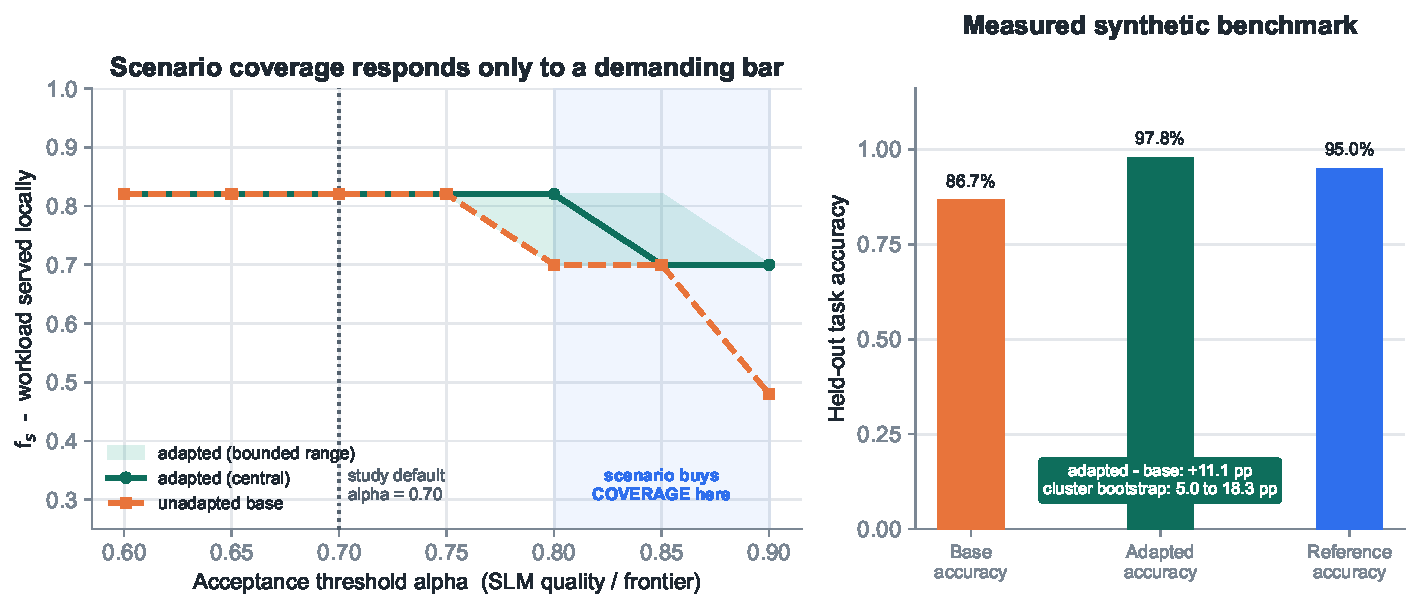
\includegraphics[width=\textwidth]{fig_quality_vs_coverage.pdf}
\caption{The two evidence boundaries in the adaptation analysis. Left:
coverage against the acceptance threshold under the inherited workload-ratio
scenario, with and without the assumed uplift. Right: measured held-out
accuracy on the public synthetic benchmark for the base, adapted and reference
models. The right panel is not a human study, a sampled workload, or an
independent device replication.}
\label{fig:quality}
\end{figure*}

The correct claim is narrower than the one we set out to test. The declared
ratios imply that adaptation would not let a local model attempt more of this
work at $\alpha = 0.70$. The public benchmark suggests that adaptation can
improve correctness on these synthetic tasks, but it does not establish that
users experience the same gain. A sampled real workload, multiple physical
device classes, and blinded human or task-specific grading remain necessary
before promoting this to a product-level quality claim.

% ===================================================================== %
\section{Amortisation}
\label{sec:amortise}

An adapter is not free. We first charge the full training run against the
per-query saving of serving locally rather than in the cloud, with two
accounting choices made deliberately against the hypothesis: training is charged
at \emph{full} device power rather than marginal, and savings are measured
against a \emph{hyperscale} cloud query, which is the cloud's best case.
\S\ref{sec:whorepays} then asks whether that saving is the adapter's to claim,
and concludes that at an ordinary acceptance threshold it is not.

\begin{table}[t]
\caption{Adaptation break-even at 50 queries/day}
\label{tab:breakeven}
\centering
\small
\begin{tabular}{lrrrr}
\toprule
\textbf{Run} & \textbf{Hours} & \textbf{kWh} & \textbf{Queries} & \textbf{Days} \\
\midrule
Persona 8B, dGPU & 0.5 & 0.21 & 140 & 3 \\
Persona 8B, APU & 3.3 & 0.43 & 288 & 6 \\
Support 7B VLM, APU & 12.4 & 1.61 & 1{,}073 & 21 \\
Capability 27B, APU & 82.1 & 10.67 & 7{,}127 & 143 \\
\bottomrule
\end{tabular}
\end{table}

Every case repays inside a year on this accounting, and three of the four inside
a month (Table~\ref{tab:breakeven}). The 27B capability run - four days of
continuous training - is repaid after about five months of ordinary use.

\subsection{Repaid to whom? A correction}
\label{sec:whorepays}
Table~\ref{tab:breakeven} charges the training run against the cloud-minus-edge
saving on \emph{every} query the adapted model then serves. Read against
\S\ref{sec:uplift}, that premise does not survive. If adaptation moves no query
across the routing boundary, those queries ran locally before the adapter
existed and their saving accrues whether or not it exists; crediting it to the
adapter counts a benefit the base model already delivered.

Charging only the coverage the adapter actually moves gives a different and
less flattering picture:

\begin{center}\small
\begin{tabular}{lrrr}
\toprule
Threshold & Coverage moved & Attributable saving & Payback \\
\midrule
$\alpha = 0.60$ & $+0\%$ & $0\Wh$/query & never \\
$\alpha = 0.70$ & $+0\%$ & $0\Wh$/query & never \\
$\alpha = 0.80$ & $+12\%$ & $0.18\Wh$/query & 3.3 years \\
$\alpha = 0.90$ & $+22\%$ & $0.33\Wh$/query & 1.8 years \\
\bottomrule
\end{tabular}
\end{center}

\noindent \textbf{At the study's own default threshold the adapter has no
energy payback at all.} It displaces nothing, because there was nothing left to
displace; its training cost is a net addition, bought for quality rather than
for footprint. Payback appears only in the regime where adaptation moves the
routing boundary, and even there it is measured in years rather than months.

The two accountings are not competing arithmetics for one quantity - they
answer different questions. Table~\ref{tab:breakeven} correctly answers ``how
long does a local deployment take to repay an adaptation run against an
all-cloud counterfactual,'' which is the right frame for a user who would have
abandoned the local model and gone to the cloud had its answers not improved:
someone whose \emph{revealed} acceptance threshold sits above the coverage knee
even though their stated one does not. That is a behavioural assumption, we
state it as one, and we report both bounds rather than choose between them.

H8 is therefore recorded as \textbf{partial and accounting-dependent}, not
validated. The two accountings answer different questions, and which one
applies is a property of the deployment rather than of the adapter.

The companion study's caveat applies on top of both readings. Payback scales
inversely with the cloud baseline being displaced; against a hyper-efficient
$0.24\Wh$ prompt rather than a $1.8\Wh$ one, every figure above lengthens by
roughly an order of magnitude.

\subsection{Money, and the surcharge that compounds}

The training bill is the smaller half of the comparison. Hosted fine-tuning
charges once for training tokens, and then may charge a persistent endpoint
premium. Our dated third-party price snapshot reports a $1.5\times$ tuned-endpoint
multiplier for three of the four entries~\cite{tuning_pricing2026}; that is a
scenario input, not a provider-wide fact, and only the cheapest entry in the
snapshot has no such premium. Over one
year at 50 queries per day, a locally adapted 27B costs \$1.71 of training
electricity plus \$0.73 of inference electricity; the cheapest hosted
equivalent costs \$7.05 of training plus \$109.50 of
inference - $\mathbf{48\times}$ the total, rising to $218\times$ against a
mid-tier hosted model. A local adapter leaves the per-query cost exactly where
it was.

% ===================================================================== %
\section{Safety, delimited}
\label{sec:safety}

Qi \emph{et al.}~\cite{qi2023finetuning} showed that fine-tuning removes safety
alignment - with ten adversarial examples for under \$0.20, and measurably even
with entirely benign data. Any product that hands users a trainer inherits this,
and we do not dispute it.

\subsection{Measured counter-evidence, and what it does not show}
\label{sec:measured}

One deployment's support model has been adapted five times, with aggregate
scores retained~\cite{autoyou_support2026}, over Qwen2.5-VL bases
\cite{qwen25vl2025}. The underlying prompts, answers, checkpoints, trainer
logs, and task-level labels are not in the public release. The report also does
not expose enough checkpoint lineage to independently verify the claimed base
pairing. We therefore retain the table only as a deployment-reported
observation, not as a reproducible experiment or a multi-model comparison. A
rank-32 LoRA over a reported 1{,}750-sample corpus produced:

\begin{center}\small
\begin{tabular}{lrr}
\toprule
& \textbf{before} & \textbf{after} \\
\midrule
Screen identification & 30.8\% & \textbf{92.9\%} \\
Refuses out-of-scope code questions & 0\% & \textbf{100\%} \\
Leaks source code & 25\% & \textbf{0\%} \\
\bottomrule
\end{tabular}
\end{center}

The capability result (E1) is a reported observation that adaptation can move a
task class on this deployment. It is not an independently verified existence
proof: the base checkpoint, task-level outputs, grader, and exact train/eval
separation are not public, and the reported parameter pairing cannot be audited
from this release.

The safety result (E2) runs opposite to \cite{qi2023finetuning}, and the reason
is instructive rather than contradictory. That corpus contains 120 refusal
samples - $6.9\%$ of it - so refusal was \emph{in the training distribution}.
Qi \emph{et al.} describe adapters that are \emph{silent} about safety: a
gradient has no reason to preserve behaviour that nothing in the corpus rewards,
so it decays. The correct generalisation is neither ``fine-tuning is safe'' nor
``fine-tuning is unsafe'' but: \textbf{fine-tuning moves whatever the corpus
specifies, in whichever direction the corpus specifies, and lets everything else
decay.}

For a locally-adapted assistant this is the difference between a hazard and a
control surface - but only if the product treats it as one. Safety cannot be
inherited by a user-trained adapter; it has to be a non-optional part of every
corpus the system assembles, plus a probe that runs before an adapter is
installed. That is a build requirement, and we record it as one.

A third finding (E3) was previously framed as a 3B-versus-7B model-selection
comparison. We withdraw that interpretation from the public result: the base
labels and checkpoint lineage are not independently auditable here. No claim
about parameter count or data being the binding constraint is made until matched
base and adapted manifests are released.

\subsection{Scope}

One deployment, one product's surface area, probe sets of 12--14 screens and 8
code probes scored by an automated judge. These are deployment-reported
observations, not independently reproducible existence proofs or effect sizes,
and nothing in this paper treats them otherwise. Aggregate scores only were
read; no prompt, answer, screenshot or user content enters the analysis.

% ===================================================================== %
\section{Forgetting and scale}
\label{sec:scale}

\subsection{C4: forgetting}

The objection that narrowing a small model destroys its general ability is
weaker than intuition suggests. Biderman \emph{et al.}~\cite{biderman2024lora}
report that LoRA learns \emph{less} in-domain than full fine-tuning and
correspondingly \emph{forgets less} out-of-domain in their evaluated settings.
We do not re-run their regularizer comparison, so the low-rank constraint is a
plausible mechanism, not a product-level guarantee. Three structural
defences add to it - the base weights are never modified, so a misbehaving
adapter is unloaded rather than un-trained; CorDA's knowledge-preserved
mode~\cite{yang2024corda} addresses the objection at initialisation; and the
unadapted hard-reasoning class continues to route out regardless.

The residual risk is real and we do not model it away: a personal corpus is
small, unbalanced and self-similar, which is the regime where over-fitting is
most likely. The mitigation is unglamorous - a held-out split and a
general-ability regression probe before installation.

\subsection{C6: does repetition lose at scale?}

The strongest form of the centralized objection is that a hyperscaler fine-tunes
once, at enormous but amortised cost, while decentralized adaptation repeats the
work for every user; at sufficient $N$, repetition must lose.

It does not, and the reason is arithmetic rather than rhetorical. Both the
training term and the inference-saving term scale linearly in $N$, so their
ratio is constant: the payback period is $12$ days at $10^5$ users and $12$ days
at $10^8$. There is no scale at which the comparison behaves differently.

The deeper answer is that the comparison is mis-specified. A central fine-tune
serving everyone is only comparable if one adapter suits everyone, and the
entire point of a persona adapter is that it encodes one person. The honest
comparison is $N$ local runs against $N$ personalised runs \emph{plus the
transfer of $N$ private corpora to a trainer} - and the second term is what
locality removes.

% ===================================================================== %
\section{Locality and the shape of the artifact}
\label{sec:transport}

Cloud fine-tuning requires the training corpus to reach the trainer. For a
persona adapter that corpus \emph{is} the user's message history, so the privacy
question is settled before any policy is written: either the messages were
uploaded or they were not. Local adaptation makes ``we never received it'' a
property of the topology rather than a promise in a document - the same class of
argument as transport-layer confidentiality, verified the same way, by what the
system is unable to do.

Adapter \emph{size} then decides whether that property survives contact with
more than one device. On an 8B model at $r{=}32$, a conventional LoRA adapter is
$174.6$\,MB and takes $70$ seconds to cross a $20$\,Mbit/s link: a file
transfer. VeRA is $2.8$\,MB and $1.1$ seconds; LoRA-XS is $0.52$\,MB and
$0.2$ seconds. Both are messages. That is the difference between personal
adapters that sync between a person's own devices as a background nicety and
personal adapters that require an explicit chore - and it is the reason the
low-parameter methods matter here despite being uninteresting on a benchmark
leaderboard.

% ===================================================================== %
\section{Threats to validity}

\textbf{One validation point.} The memory model is checked against a single
publicly documented run. It reproduces that run to $-0.6\%$, which is evidence that the
terms are right, not that the model generalises across architectures. MoE
models in particular are not validated and their activation term differs.

\textbf{Synthetic benchmark and residual scenario.} The public multi-model
evaluation replaces the $+2/+6/+14$ point range for the narrower estimand of
held-out four-choice task accuracy. It uses 20 evaluation tasks in each of
five synthetic classes, three adapter seeds and three model clusters on one
CPU-only physical host. The $+\AdaptationUplift\pp$ estimate has an exact
cluster sign-flip $p=\AdaptationClusterP$; this is not enough clusters for a
strong generalisation claim. Hard reasoning supplies most of the gain, while
extraction and retrieval are saturated at 100\% in this task set. The old
range is retained only as a routing sensitivity scenario, not as an empirical
effect size. The workload-weighted $88.4\% \rightarrow 93.9\%$ figure is still
a \emph{consequence} of that scenario rather than evidence for it.

The task identifiers are disjoint, but the public generator reuses a small
set of class templates and the same four-choice response format across the
training and evaluation splits. A supplemental prompt-surface holdout changes
the surrounding wording and reports $\AdaptationHoldoutBaseAccuracy\%$ to
$\AdaptationHoldoutAdaptedAccuracy\%$ ($+\AdaptationHoldoutUplift\pp$), but it
reuses the same semantic records and tests only one paraphrase. It therefore
weakens the exact-template explanation without distinguishing semantic transfer
from memorisation of records, answer labels, recurring class structure, or
contamination. A separate new-semantic holdout now uses fresh records and
formats and reports $\AdaptationSemanticBaseAccuracy\%$ to
$\AdaptationSemanticAdaptedAccuracy\%$ ($+\AdaptationSemanticUplift\pp$),
with a model-cluster interval from $\AdaptationSemanticUpliftLow\pp$ to
$+\AdaptationSemanticUpliftHigh\pp$ and exact $p=\AdaptationSemanticClusterP$.
Its model-level directions are mixed, which weakens broad transfer claims, but
it remains synthetic, one-host, automatically graded, and does not include a
contamination or untouched general-ability probe. Semantic transfer and
product-level quality therefore remain unresolved.

\textbf{The workload mix is inherited, not measured.} $\fs$, the class weights,
and the base capability ratios all come from the companion study, where they are
themselves modelling choices compared with NVIDIA's reported agentic
replaceability range rather than against a task corpus of our own. A different
workload composition - one weighted toward hard reasoning, or toward tasks whose
base ratio sits just below $\alpha$ - would change both results here, and the
second case would make adaptation buy coverage at the default threshold. We
report the sensitivity of the knee for exactly this reason, but we cannot bound
the sensitivity to a workload we did not sample.

\textbf{Energy corpus and cloud baselines.} The companion study provides primary
2026 consumer GPU board measurements ($\RtxThreeEnergy\Wh$ for 3B and $\RtxEightEnergy\Wh$ for 8B on
an RTX 5070), but no peer-reviewed whole-system per-query measurement covers
the 2026 frontier or the 2026 open-weights tier under identical prompts. Hosted
pricing, open-weights architectures and adapter evaluations are current to
September 2026; fleet cloud comparisons remain literature-derived estimates.

\textbf{Limited replication.} \S\ref{sec:measured} is one team's five runs on
one product, and the public benchmark uses three model clusters on one
physical host. Neither can estimate a population effect, independent-device
reproducibility, human quality, or generality across products.

\textbf{Already-owned hardware only.} Every result assumes the device exists for
other reasons. The companion study establishes that embodied carbon dominates
for a device provisioned specifically for inference; nothing here is an argument
for buying an APU.

% ===================================================================== %
\section{Conclusion}

One public community recipe demonstrates parameter-efficient adaptation on
already-owned consumer hardware for a 27B-class model. Under the declared
cost model, it is $48$--$218\times$ cheaper over one year than the hosted
equivalent - chiefly because hosted personalisation surcharges every
subsequent query, permanently, while a local adapter does not.

Its \emph{energy} case is weaker than it first appears, and the weakness is
instructive. Against an all-cloud counterfactual an adaptation run repays inside
a year in every case modelled. Against the routing it actually changes, it
repays nothing at an ordinary acceptance threshold, because at that threshold it
changes no routing. An adapter is an instrument for quality, and treating it as
an instrument for footprint requires a behavioural assumption that should be
argued rather than assumed.

What the declared model buys is not what we expected. At an ordinary acceptance
threshold it adds no coverage, conditional on the chosen ratios and workload.
The public synthetic benchmark measures a $+\AdaptationUplift\pp$ increase in
held-out task accuracy, but the result is limited by three model clusters, one
physical host, deterministic synthetic tasks and automated choice grading.
The supplemental prompt-surface probe remains positive at
$+\AdaptationHoldoutUplift\pp$, but reuses the same records and therefore does
not resolve semantic-transfer, contamination, or independent-replication
counterclaims.
The new-semantic holdout is only $+\AdaptationSemanticUplift\pp$, with a
model-cluster interval from $\AdaptationSemanticUpliftLow\pp$ to
$+\AdaptationSemanticUpliftHigh\pp$ and exact $p=\AdaptationSemanticClusterP$.
Its mixed model directions mean that broad semantic transfer is not
established by the current evidence.
Coverage is bought only by users who demand frontier-comparable quality in the
inherited scenario, and hard reasoning remains unreachable under the stated
adaptation boundary.

The practical consequence for a system builder is the inverse of the intuition:
adapt to raise the standard of what you already serve locally, not to widen what
you attempt. A router that treats an installed adapter as licence to keep more
work on the device will, on this model, keep the wrong work.

The private observation we did not anticipate is the safety one. Fine-tuning is
neither safe nor unsafe by construction: it can move what the corpus specifies
while other behavior changes or decays. That makes the corpus, not the recipe,
the safety-critical artifact in a system that lets people teach their own
assistant - and it makes an explicit refusal distribution and a pre-installation
probe the two things such a system should not ship without. This remains an
existence observation until independent products, devices and task-specific
graders reproduce it.

\section*{Reproducibility}
All analytical routines, simulation models, dataset parameters and
figure-generation pipelines supporting this work form a single deterministic
pipeline requiring only standard scientific libraries, and produce the
parameter rosters, Monte-Carlo sweeps and sensitivity curves without relying
on proprietary cloud APIs. All of it is released openly under an MIT
licence~\cite{autoyou2026measure}.

One class of input is deliberately not redistributable. The deployment adapter
artifacts behind \S\ref{sec:measured} come from a deployed assistant whose
training corpus and evaluation transcripts contain product and user material,
and only aggregate scores were ever extracted from them
\cite{autoyou_support2026}. Those aggregates are not redistributable, so that
deployment observation cannot be independently reproduced, and H11 remains
\emph{not independently validated}. The public synthetic benchmark is a
separate, reproducible replacement for the narrow task-accuracy estimand: its
task manifest, aggregate task-level scores, adapter files, model revisions and
runtime record are released beside this manuscript. We prefer a result the
reader can see is limited over one that looks reproducible and is not. Every
other number in this paper is recomputed from the parameters and measurement
records described above.

The prompt-surface holdout is released separately with its task manifest,
aggregate task-level scores, adapter references, model revisions and runtime
record. It is a robustness probe over the same public evaluation records and
must not be counted as an independent device or workload replication.

The new-semantic holdout is released separately with its fresh task manifest,
aggregate task-level scores, adapter references, model revisions and runtime
record. It is a distribution-shift check over synthetic records, not an
independent device replication or a sampled user workload.

This is research release v0.3.0 dated 2026-09-14. Venue and DOI metadata are
intentionally unassigned in this release. The public multi-model adaptation
score file is present and reports a measured synthetic-task accuracy result;
the $+2/+6/+14$ scenario is not promoted to an empirical effect size for that
benchmark. Repository metadata, the citation audit, and the follow-up protocol
for sampled workloads and independent device replication are released beside
this manuscript.

\bibliographystyle{IEEEtran}
\bibliography{references}

\end{document}
